\documentclass[10pt,a4paper]{article}
\usepackage[margin=20mm]{geometry}
\usepackage[T1]{fontenc}
\usepackage{lmodern,amsmath,amssymb,graphicx,booktabs}
\usepackage[numbers]{natbib}
\usepackage[hidelinks]{hyperref}
\usepackage[font=small,labelfont=bf]{caption}
\setlength{\textfloatsep}{8pt plus 2pt minus 2pt}
\setlength{\intextsep}{8pt plus 2pt minus 2pt}
\graphicspath{{../figures/}}
\newcommand{\Oh}{\mathrm{Oh}}
\newcommand{\Rmin}{R_{\min}}
\title{Finite-Ohnesorge validation of drop coalescence}
\author{CoMPhy Lab}
\date{3 October 2026}

\begin{document}
\maketitle

Finite inertia slows the coalescing neck before the neck reaches the expected
inertial crossover. At $\Oh=0.6$, the present finite-element method (FEM)
reproduces the developed velocity curve of Anthony, Harris and
Basaran~\cite{Anthony2020}, while its velocity lies below the present Stokes
solution by 6.46\% at $\Rmin=10^{-5}$ and 12.15\% at $\Rmin=0.03$.
We keep comparison with published data separate from numerical verification
and convergence. An independent Stokes boundary-integral method (BIM)
reproduces the FEM startup where the published Stokes markers differ.

\begin{figure}[!ht]
\centering
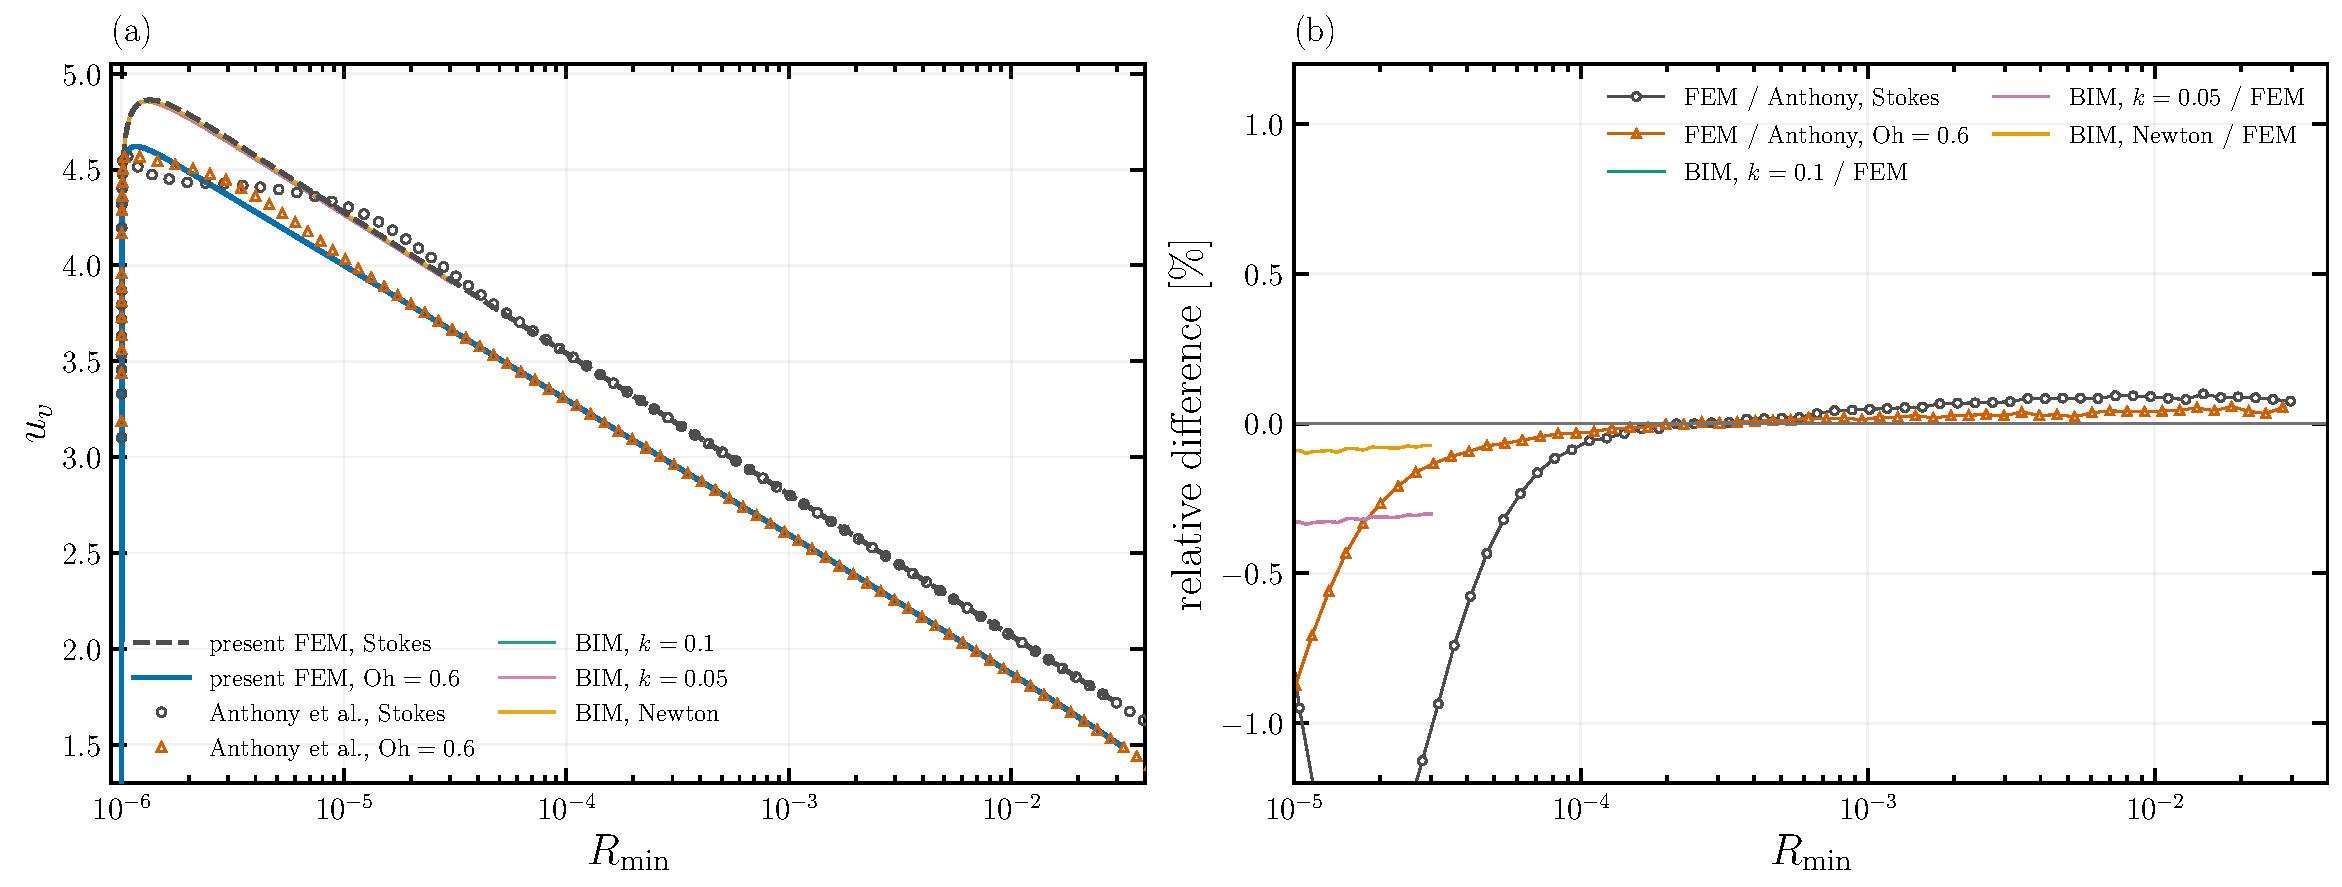
\includegraphics[width=\linewidth]{public-validation-overview-v4.pdf}
\caption{Neck velocity in visco-capillary units. Blue: present FEM at
$\mathrm{Oh}=0.6$; dashed grey: Stokes FEM. Triangles and circles: Anthony
et al.'s finite-Oh and Stokes markers. Green, pink and yellow: independent
Stokes BIM. Panel (b) compares FEM/Anthony and BIM/FEM minus one in per
cent at equal radius, without fitted offsets; early startup is shown
separately in Figure~\ref{fig:bim}.}
\label{fig:overview}
\end{figure}


\section{Problem and scales}
Two equal drops of radius $R_d$ coalesce in a passive exterior of zero
density and viscosity. Length, velocity and time scales are $R_d$,
$\gamma/\mu$ and $\mu R_d/\gamma$. With
$\Oh=\mu/\sqrt{\rho\gamma R_d}$, the liquid obeys
\begin{equation}
\Oh^{-2}(\partial_t\boldsymbol{u}+\boldsymbol{u}\cdot\nabla\boldsymbol{u})
=\nabla\cdot\boldsymbol{\sigma},\qquad
\nabla\cdot\boldsymbol{u}=0,\qquad
\boldsymbol{\sigma}=-p\boldsymbol{I}+\nabla\boldsymbol{u}+\nabla\boldsymbol{u}^{T}.
\end{equation}
The initial bridge has $R_0=10^{-6}$ and $Z_0=R_0^2/2$; its meridian
$[r-(R_0+Z_0)]^2+z^2=Z_0^2$ joins the spherical drop tangentially.
The finite-Oh drops start from rest. The FEM uses Taylor--Hood triangles,
tip-graded ALE coordinates and second-order backward differentiation.

The solver time $t_v$ is already visco-capillary. We construct
$\tau_v=t_v+t_{\mathrm{con},v}$ by fitting
$\Rmin=A(t_v+t_{\mathrm{con},v})^n$ over $10R_0\leq\Rmin\leq100R_0$,
following the contact-time extrapolation of Ref.~\cite{Anthony2020}.
The contact shifts are $1.5202\times10^{-7}$ at $\Oh=0.6$ and
$1.4309\times10^{-7}$ in Stokes flow. No additional division by Oh is
made, and no offset is fitted to the published markers.

\clearpage
\section{FEM against Anthony et al.}
\begin{figure}[!ht]
\centering
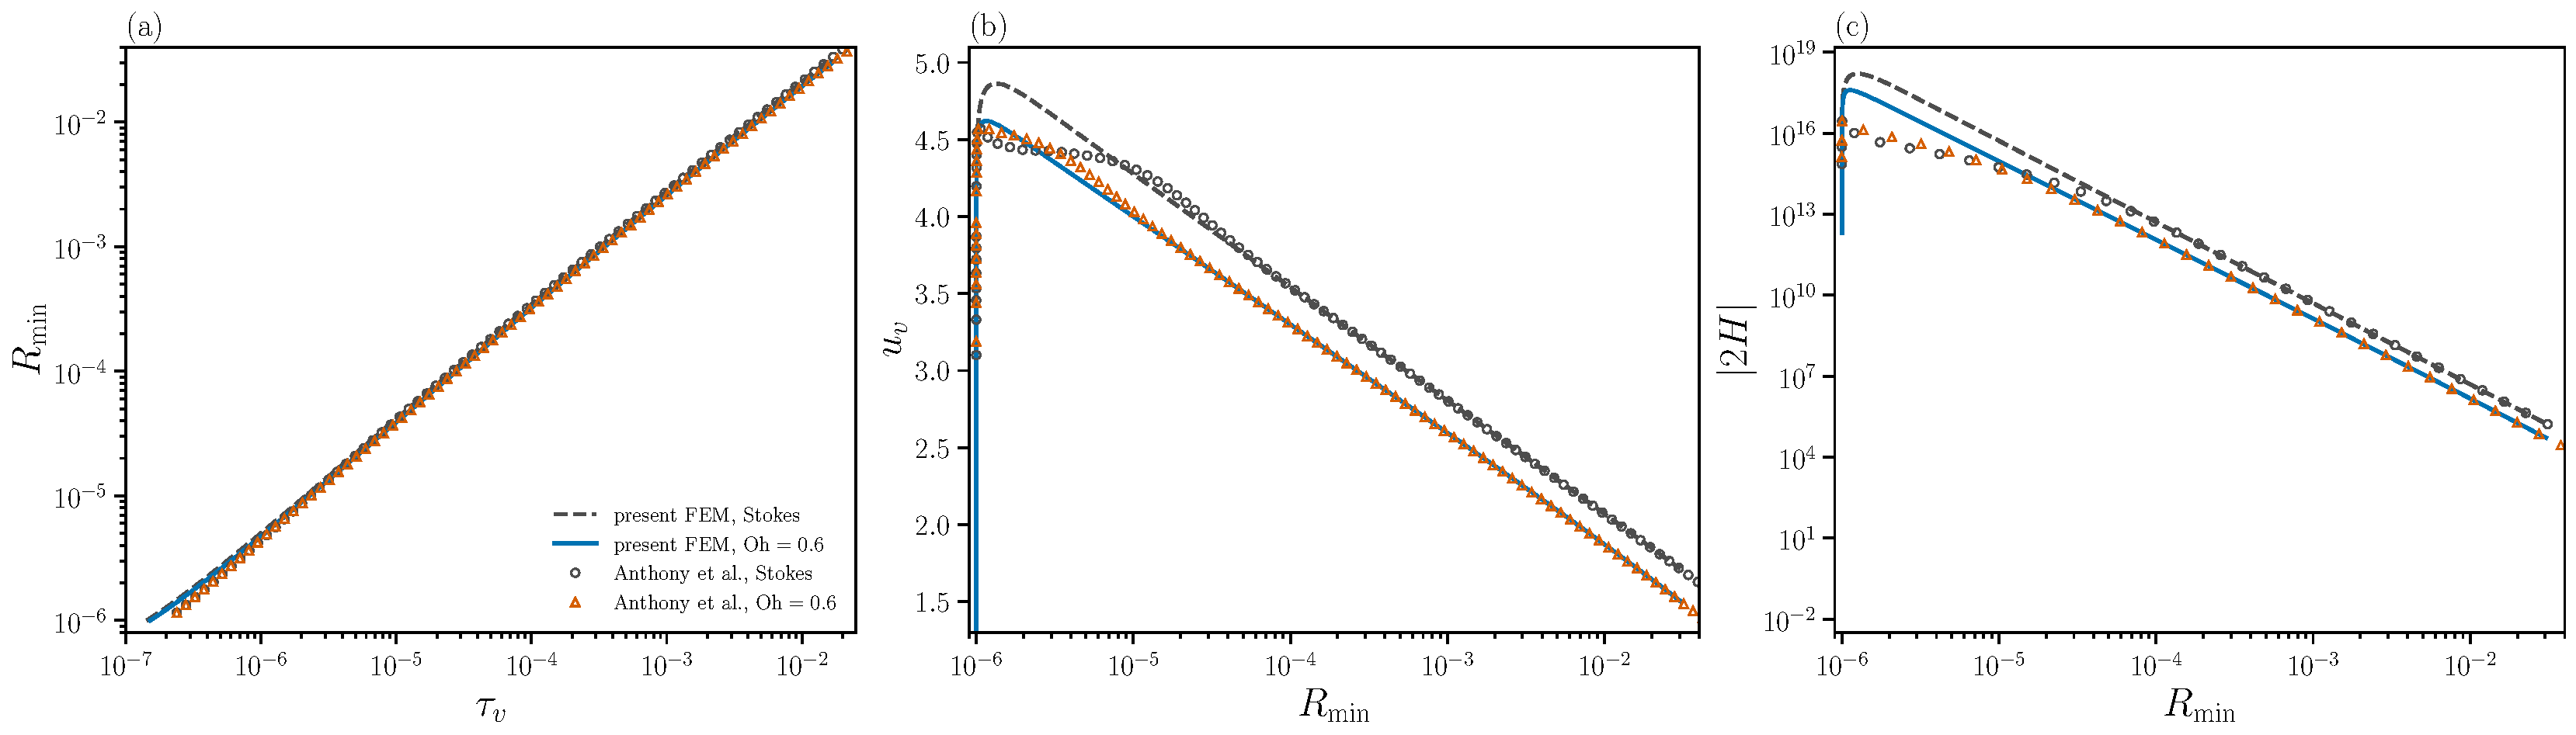
\includegraphics[width=\linewidth]{finite-oh06-validation-v3-anthony.pdf}
\caption{Both FEM curves and both digitised series from Anthony
et al.~\cite{Anthony2020}, Fig. 3: (a) radius against viscous coalescence
time, (b) velocity against radius and (c) magnitude of twice the mean
curvature against radius. Colours and markers follow
Figure~\ref{fig:overview}. The power-law contact-time construction
affects (a) only. No marker-fitted offsets are used.}
\label{fig:anthony}
\end{figure}


The median differences $100(\mathrm{FEM}/\mathrm{Anthony}-1)$ are listed
below. The bands refer to $\tau_v$ for radius and $\Rmin$ for velocity
and curvature. Markers outside the computed coverage are excluded.
\begin{center}
\small
\begin{tabular}{llrrrr}
\toprule
Quantity & Abscissa & $10^{-5}$--$10^{-4}$ & $10^{-4}$--$10^{-3}$ & $10^{-3}$--$10^{-2}$ & $\geq10^{-2}$ \\
\midrule
$\Rmin$ & $\tau_v$ & $+0.062\%$ & $-0.023\%$ & $-0.029\%$ & $-0.033\%$ \\
$u_v$ & $\Rmin$ & $-0.133\%$ & $+0.005\%$ & $+0.028\%$ & $+0.044\%$ \\
$\lvert2H\rvert$ & $\Rmin$ & $+3.19\%$ & $-3.50\%$ & $-3.04\%$ & $-3.37\%$ \\
\bottomrule
\end{tabular}
\end{center}
For $\Rmin\geq10^{-4}$, velocity differences range from $-0.027\%$ to
$+0.057\%$. Developed curvature is approximately 3--4\% lower.
The preceding curvature band is still transient: differences span
$-3.86\%$ to $+73.31\%$. The earliest finite-Oh velocity markers differ
by up to about 3.8\%; the radius comparison is also contact-time sensitive.
We do not extend developed-range agreement to startup.

\section{Verification and convergence}
The inertial normal-mode test gives frequency errors of $-0.044\%$ and
$-0.019\%$ at 200 and 400 steps per period. The $\Oh=10^{12}$ limit
reproduces Stokes steps to $10^{-14}$ relative. The finite-Oh reference
reaches $\Rmin=0.03037$ in 878 steps and 133 remeshes; its relative
volume drift is $2.85\times10^{-7}$.

At $R_0=10^{-3}$ the frame checks differ by at most approximately 0.045\%.
The tip-map and half-time-step checks have 95th-percentile absolute
differences below 0.003\%, not uniform maximum errors.
Bulk-grading 0.07 and remesh-growth 1.05 partners remain outstanding;
we do not claim complete finite-Oh mesh and remeshing convergence.
\begin{figure}[!ht]
\centering
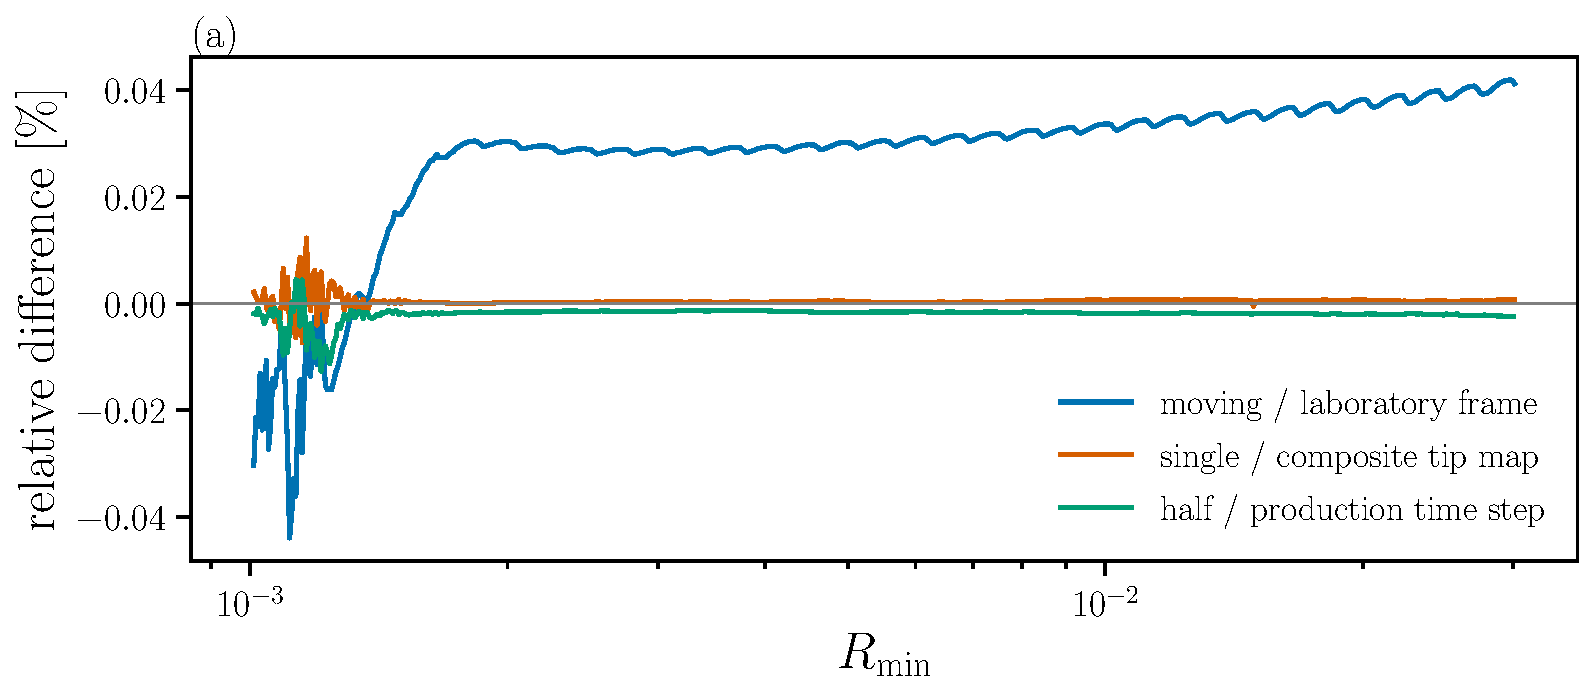
\includegraphics[width=0.68\linewidth]{finite-oh06-validation-v3-convergence.pdf}
\caption{Completed finite-Oh frame, tip-map and time-step checks at
$R_0=10^{-3}$, compared at equal radius from $1.01R_0$. Blue: moving
versus laboratory frame; orange: single versus composite tip map;
green: half versus production time step on the same single map.
Bulk-grading and remeshing partners remain outstanding.}
\label{fig:convergence}
\end{figure}


\clearpage
\section{Independent Stokes BIM}
\begin{figure}[!ht]
\centering
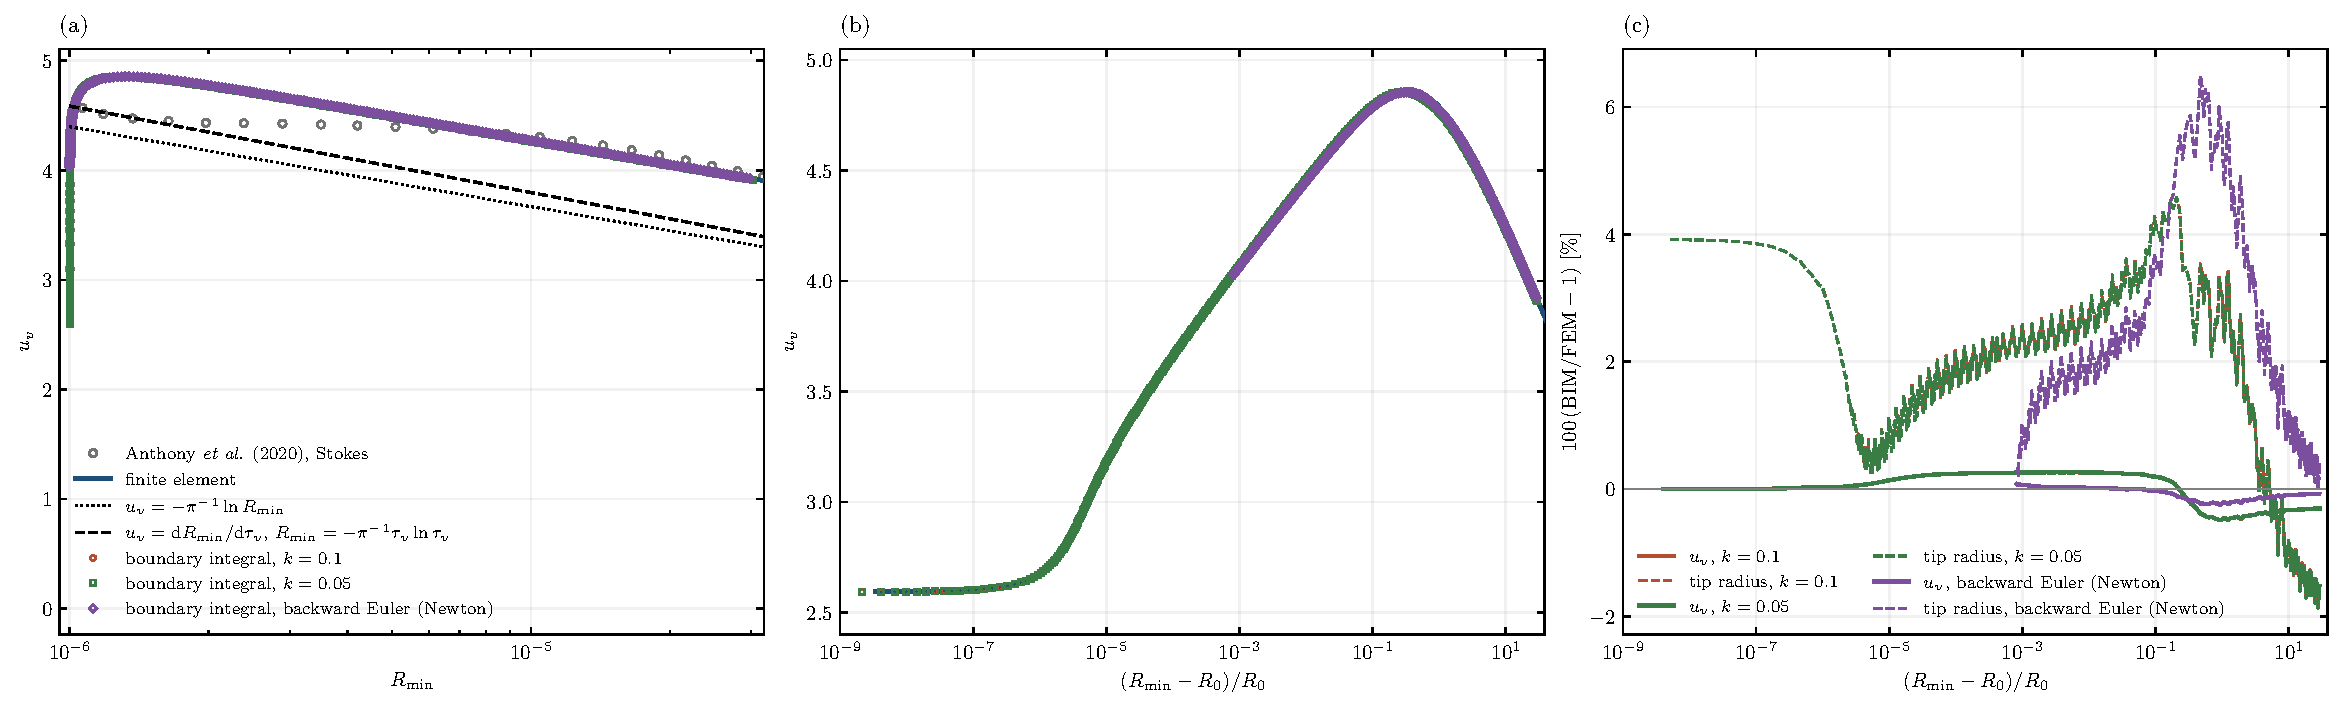
\includegraphics[width=\linewidth]{stokes-bim-fem-anthony-startup.pdf}
\caption{Independent Stokes BIM, Stokes FEM and Anthony's Stokes
startup for $R_0=10^{-6}$. The backward-Euler Newton series is within
0.243\% of FEM; the linearly implicit grading series are within
approximately 0.489\%. Velocity is the discriminating observable;
tip-curvature estimators carry approximately 4\% uncertainty. This
comparison contains no independent inertial BIM calculation.}
\label{fig:bim}
\end{figure}


The independently implemented FEM and BIM agree through the Stokes startup
peak for the same initial bridge. The BIM solves a Stokes integral equation
on a spline meridian; it does not borrow FEM fields or pressure data.
The backward-Euler Newton series differs from FEM by at most 0.243\%,
and the two linearly implicit grading series by at most approximately
0.489\%. The gradings agree much more closely with each other.
This is code-to-code verification of Stokes flow, not a second validation
of finite inertia. There is no additional independent finite-Oh boundary
solver in the present comparison. The cause of the difference from
Anthony's Stokes startup is not established here.

\section{Initial-radius independence}
\begin{figure}[!ht]
\centering
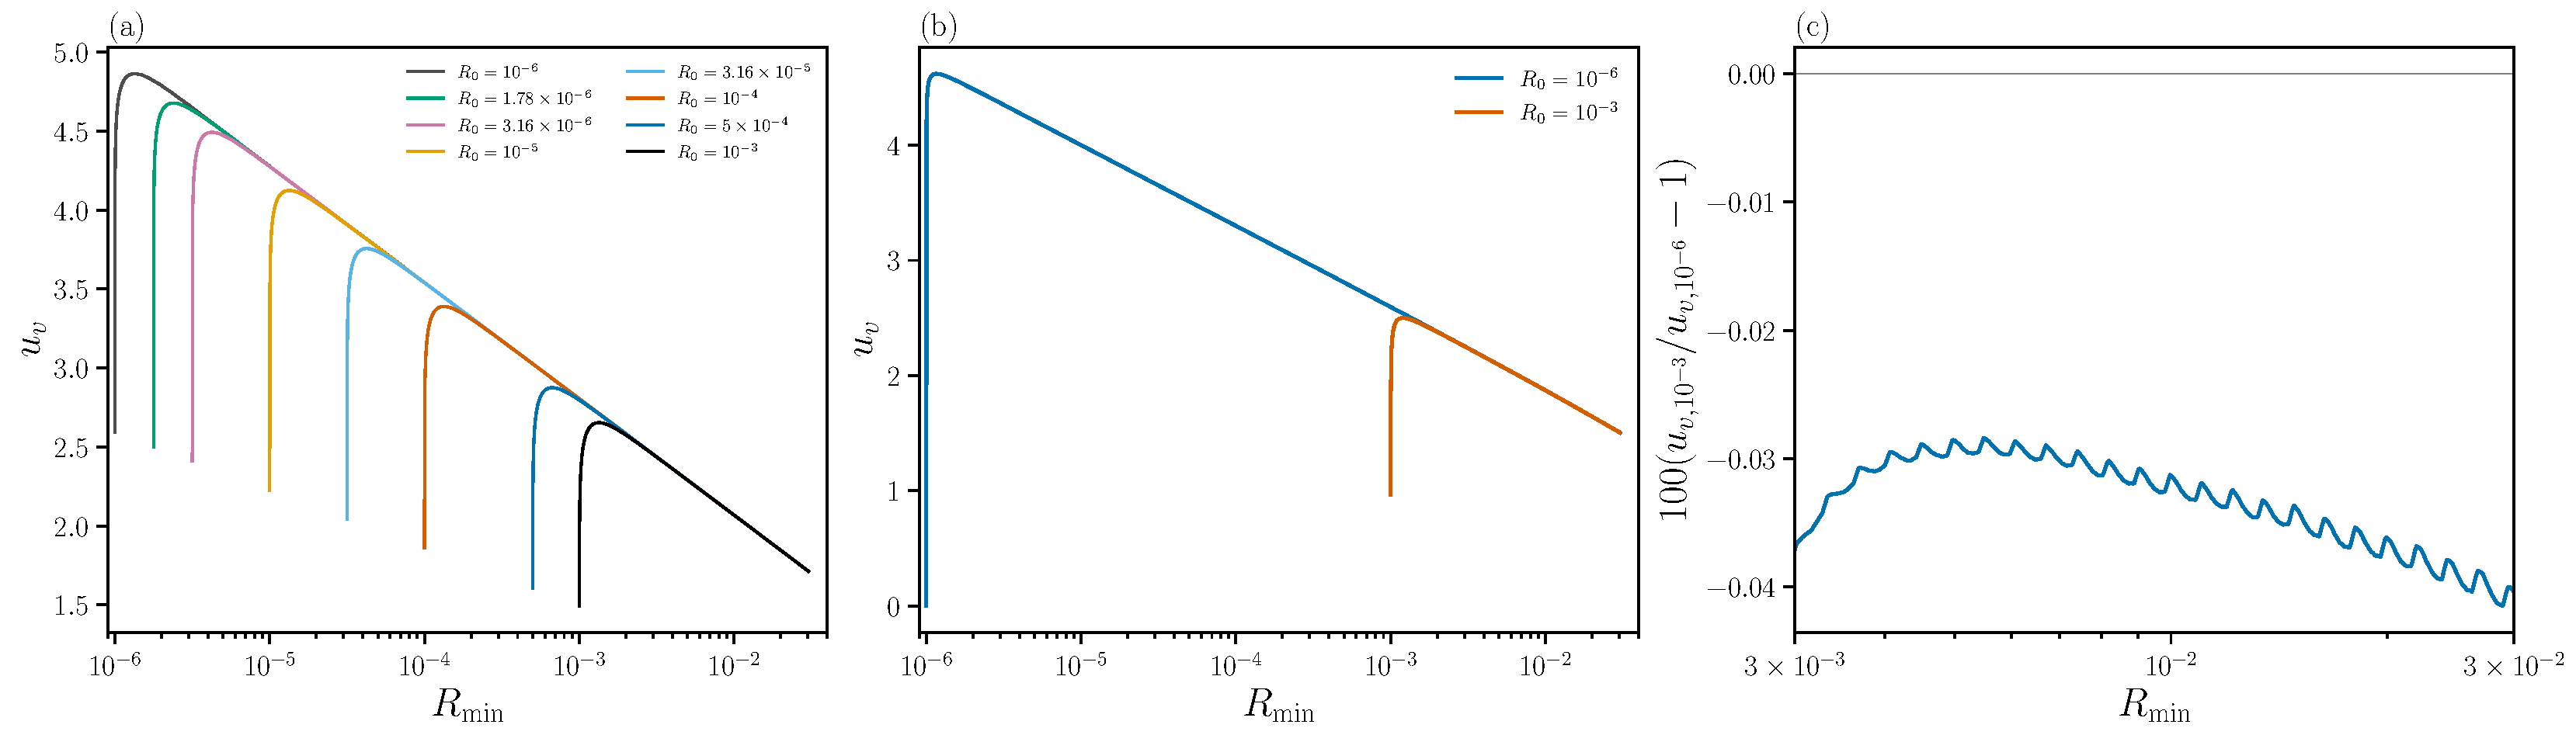
\includegraphics[width=\linewidth]{finite-oh06-validation-v3-r0.pdf}
\caption{(a) Eight Stokes initial radii from $10^{-6}$ to $10^{-3}$;
(b) the two finite-Oh endpoint radii; (c) their velocity difference
at equal radius. At $\mathrm{Oh}=0.6$, the histories agree within
0.042\% for $R_{\min}\geq3\times10^{-3}$, without offsets. The
finite-Oh intermediate-radius family is not yet complete.}
\label{fig:r0}
\end{figure}

The eight Stokes histories join the smallest bridge's curve within 0.1\%
by approximately $2.3$--$2.7R_0$. At $\Oh=0.6$, the two endpoint radii
$R_0=10^{-3}$ and $10^{-6}$ agree to within 0.042\% for
$\Rmin\geq3\times10^{-3}$. Intermediate finite-Oh radii have not yet
been computed. This two-radius check is distinct from the completed
Stokes family.

\clearpage
\section{Finite inertia relative to Stokes}
\begin{figure}[!ht]
\centering
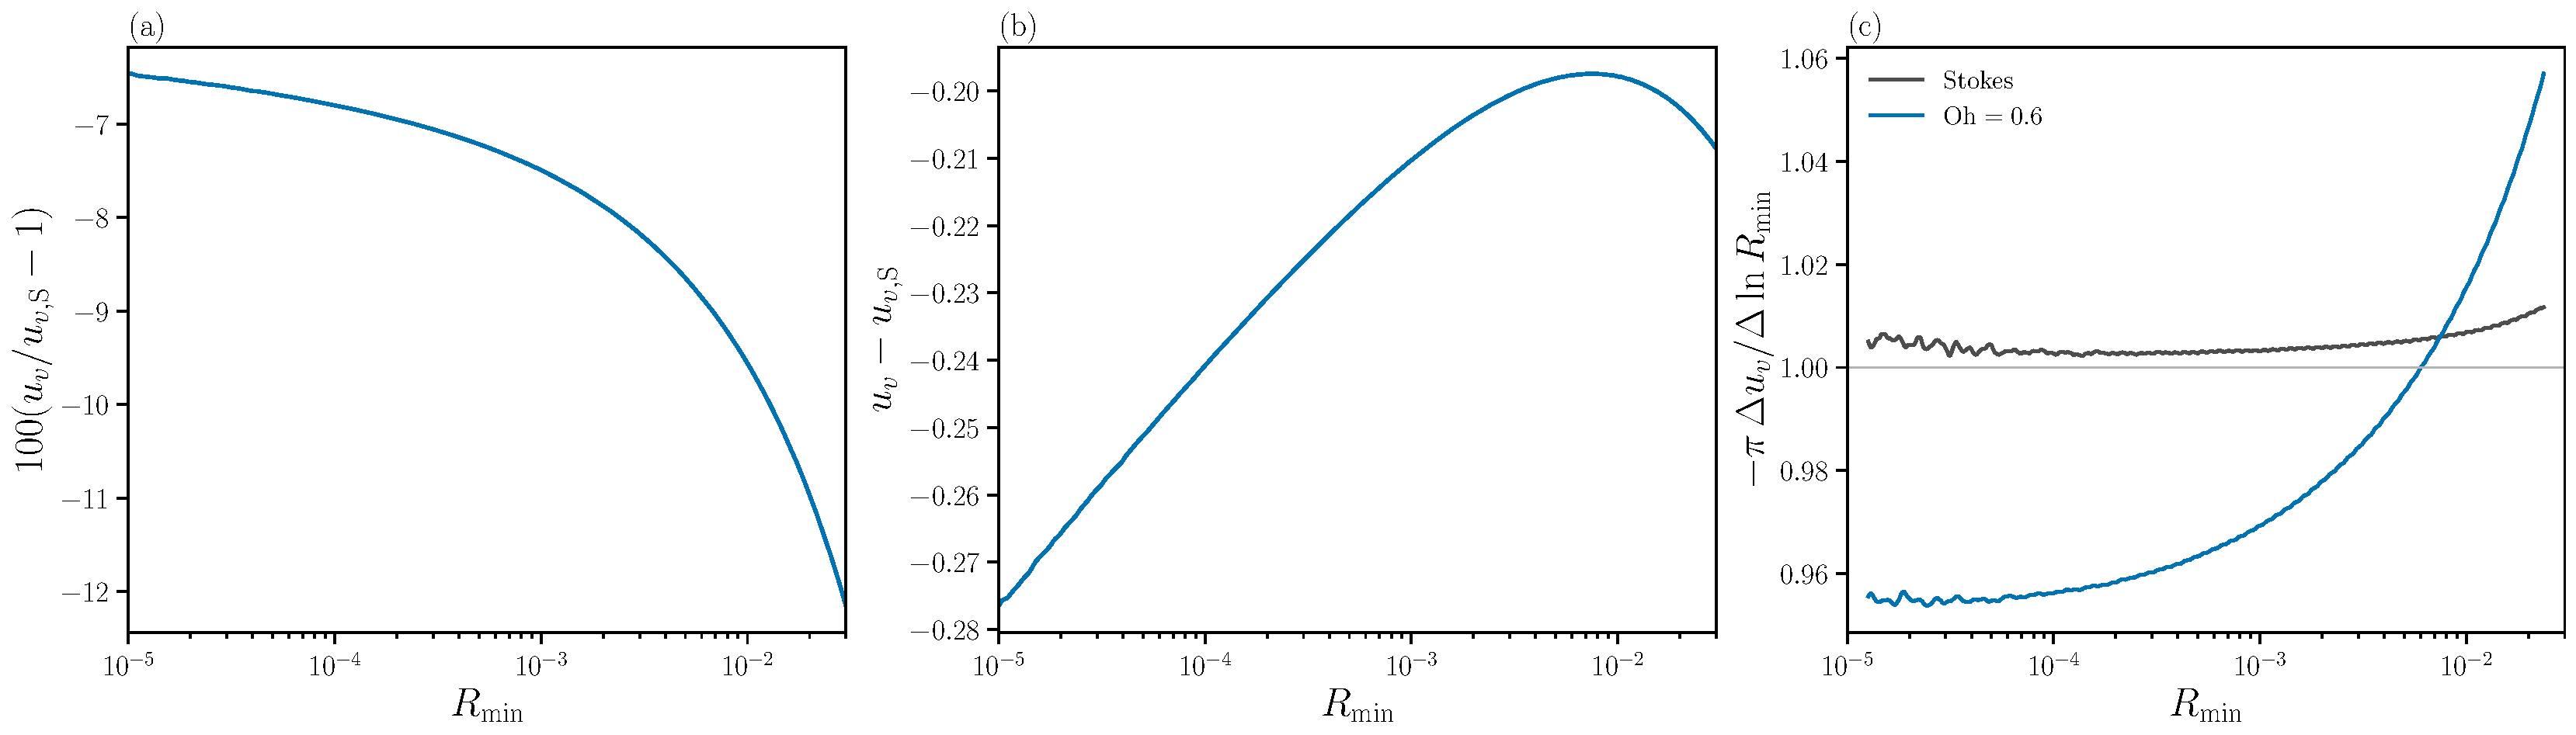
\includegraphics[width=\linewidth]{finite-oh06-validation-v3-deficit.pdf}
\caption{Finite-Oh velocity deficit at equal radius: (a) relative,
(b) absolute and (c) local logarithmic slopes normalized by $1/\pi$,
measured using secants across 0.2 decades. Grey: Stokes; blue:
$\mathrm{Oh}=0.6$. The relative deficit grows from 6.46\% at
$R_{\min}=10^{-5}$ to 12.15\% at $0.03$.}
\label{fig:deficit}
\end{figure}

At equal neck radius, the finite-Oh velocity deficit is
\begin{center}
\begin{tabular}{rrrr}
\toprule
$\Rmin$ & $\Rmin/\Oh$ & $u_v-u_{v,\mathrm{S}}$ & Relative difference \\
\midrule
$10^{-5}$ & $1.67\times10^{-5}$ & $-0.2765$ & $-6.46\%$ \\
$10^{-4}$ & $1.67\times10^{-4}$ & $-0.2408$ & $-6.80\%$ \\
$10^{-3}$ & $1.67\times10^{-3}$ & $-0.2103$ & $-7.49\%$ \\
$10^{-2}$ & $1.67\times10^{-2}$ & $-0.1979$ & $-9.56\%$ \\
$0.03$ & $0.05$ & $-0.2086$ & $-12.15\%$ \\
\bottomrule
\end{tabular}
\end{center}
The absolute deficit remains approximately $-0.28$ to $-0.20$; its relative
magnitude grows because the Stokes velocity falls. Writing
$u_v=\pi^{-1}\ln(C/\Rmin)$ defines the diagnostic
$C_{\mathrm{eff}}=\Rmin\exp(\pi u_v)$. The inferred finite-Oh/Stokes
ratio is 0.4196 at $\Rmin=10^{-5}$, 0.5371 at $10^{-2}$ and 0.5193 at
$0.03$. The first-decade median is approximately 0.444.
The finite-Oh logarithmic slope, normalized by $1/\pi$, has decade
medians of approximately 0.955, 0.961 and 0.985 between $10^{-5}$ and $10^{-2}$.

A changed outer cut-off of the Stokes logarithm is therefore plausible,
but a single constant shift cannot describe the weak slope change.
The present history reaches only $\Rmin/\Oh=0.05$ and does not test the
crossover at $R_c\approx\Oh$. An Oh ladder reaching that scale is needed
to distinguish the cut-off interpretation from other finite-inertia
corrections.

\section{Reproducibility}
The accompanying repository page records the build commands, registered
run lists and source checksums. A compact plot-input bundle permits
reproduction without raw meshes or field histories. The scripts retain
the original visco-capillary time, exclude extrapolation and emit the
comparison statistics separately from the figures. All six figure
environments have reusable TeX sources; graphics use embedded fonts.

\bibliographystyle{unsrtnat}
\bibliography{references}
\end{document}
